\documentclass{beamer}
\usetheme{AnnArbor}
\usecolortheme{beaver}
\geometry{paperwidth=140mm,paperheight=105mm}
\usepackage[utf8]{inputenc}
\usepackage[T1]{fontenc}
\usepackage[italian]{babel}
\usepackage{soul}
\usepackage{graphicx}
\usepackage{algorithm2e}
\usepackage{multirow}

\usepackage{fancyvrb}
\definecolor{felinesrcbgcolor}{rgb}{1,1,0.85}
\definecolor{felinesrcbgcolor}{rgb}{0.94,0.97,1}
\definecolor{felineframe}{rgb}{0.79,0.88,1}
\definecolor{myorange}{rgb}{1,0.375,0}
\fvset{frame=lines,
  framesep=3mm,
  framerule=3pt,
  fontsize=\small,
  rulecolor=\color{myorange},
  formatcom=\color{DarkGreen},
}

\hypersetup{
	urlcolor=myorange
}

\title[Arch2013] % (optional, only for long titles)
{Architettura degli elaboratori 2012/2013}
\subtitle{Aritmetica binaria: Operazioni con i Float}
\author{Michele ``Jazzinghen'' Bianchi\inst{1}}
\institute[DISI] % (optional)
{
  \inst{1}%
  Dipartimento di Ingegneria e Scienze dell'Informazione\\
  Universtià degli Studi di Trento
}
\date[2013-03-13] % (optional)
{13 Marzo 2013}
\subject{Computer Science, Embedded Systems}

\begin{document}
	\frame{\titlepage}
	\section{It's answer TIME!}
	\begin{frame}
    \frametitle{Alcune cose prima d'iniziare}
    \framesubtitle{Ve l'avevo detto che avrei risposto}
		\begin{itemize}
			\item Sul sito è presente il codice in C per un'applicazione che vi
				mostra la struttura in bit di un single passato via comand line.
			\item Il segno di un numero signed può venir cambiato facendo il complemento a 2
			\item L'algoritmo di Booth è un po' incasinato. Rivediamolo...
		\end{itemize}
	\end{frame}   
   
	\begin{frame}
    \frametitle{Alcune cose prima d'iniziare}
    \framesubtitle{Booth Algoritm}
		\begin{columns}
    \column{.6\textwidth}
			\begin{itemize}
				\item Scorrere un bit alla volta, controllando quello alla sua destra
				\item In base alla coppia bisognerà riportare un valore differente, shiftato in
					base al bit preso in considerazione:
				\begin{itemize}
					\item 00 o 11: Nulla
					\item 10: sommare il complemento a 2 del primo termine
					\item 01: sommare il primo termine
				\end{itemize}
				\item Finiti i bit basta sommare tutti i termini
			\end{itemize}
		\column{.4\textwidth}
			\begin{center}
	    		\includegraphics[width=.9\textwidth]{IMGs/FastBooth.png}
	    \end{center}
	  \end{columns}
	\end{frame}   
	\section{Riassunto dell'ultima puntata}  
  \begin{frame}
    \frametitle{Cos'è successo l'ultima volta?}
		Abbiamo visto:    
    \begin{itemize}
    		\item Operazioni con i signed
    		\item Rappresentazione dei numeri decimali con Fixed Point
    		\item Limite della rappresentazione Fixed Point
    		\item Rappresentazione dei numeri decimali con Floating Point
    		\item Conversione in Floating Points
    \end{itemize}
    %Unari, Babilonesi, Romani, Posizioniali (indiani), Binaria
  \end{frame}
	
	\section{Float Operations}
	\subsection{Idea di base}
  \begin{frame}
    \frametitle{Floating Point}
    \framesubtitle{Idea di base}
    In teoria le operazioni tra floating point sono molto semplici:
    $$x +_{f} y = round(x + y)$$
    $$x *_{f} y = round(x * y)$$
    
		\vspace{2em}    
    
    Più precisamente:
    \begin{itemize}
    		\item Calcolare il risultato preciso
    		\item Normalizzare la mantissa
    		\item Mettere a posto il resto
    		\begin{itemize}
    			\item Andare in overflow se l'esponente è troppo grande
    			\item Arrotondare se ci sono troppi bit nella mantissa
    		\end{itemize}
    \end{itemize}
  \end{frame}
  
  \subsection{Arrotondamento}
  \begin{frame}
	    \frametitle{Floating Point}
	    \framesubtitle{Arrotondamento}
	    Il medoto standard per i float è l'even rounding: in caso di valore in bilico arrotondare
	    in modo che la cifra meno significativa sia pari.
	    \begin{itemize}
	    		\item Più facile da implementare a livello hardware
	    		\item Migliore a livello statistico in caso di operazioni multiple su più numeri arrotondati
	    		\begin{itemize}
	    			\item I risultati con valori arrotondati per eccesso sono sovrastimati
	    			\item Quelli per difetto sottostimati
	    		\end{itemize}
	    \end{itemize}
	    
	    \pause
	    \vspace{2em}
	    
	    Ad esempio (arrotondando al millesimo):
	    \begin{center}
	    		\begin{tabular}{ccl}
	    		23.432500001 & 23.433 & [Arrotondato per eccesso] \\ 
	    		23.432499999 & 23.432 & [Arrotondato per difetto] \\ 
	    		23.432500000 & 23.432 & [A metà, pari, arrotondato per difetto] \\ 
	    		23.433500000 & 23.434 & [A metà, dispari, arrotondato per eccesso] \\ 
	    		\end{tabular} 
	    \end{center}
	  \end{frame}

  \begin{frame}
    \frametitle{Floating Point}
	  \framesubtitle{Arrotondamento binario}
		L'arrotondamento in binario funziona nella stessa maniera:
		\begin{itemize}
			\item Un numero binario è \emph{pari} se la cifra meno significativa è $0$
			\item Un numero binario è \emph{in bilico} se dopo la cifra da arrotondare troviamo
				$10\text{...}0_{2}$
		\end{itemize}
		\pause		
		\vspace{2em}
		Ad esempio (arrotondando all'1/8):
	    \begin{center}
	    		\begin{tabular}{ccl}
	    		$10.01101110_{2}$ & $10.011_{2}$ & [Arrotondato per difetto] \\ 
	    		$10.01110101_{2}$ & $10.100_{2}$ & [Arrotondato per eccesso] \\ 
	    		$10.01110000_{2}$ & $10.100_{2}$ & [A metà, pari, arrotondato per difetto] \\ 
	    		$10.01010000_{2}$ & $10.010_{2}$ & [A metà, dispari, arrotondato per eccesso] \\ 
	    		\end{tabular} 
	    \end{center}
  \end{frame}
  \subsection{Moltiplicazione}
  \begin{frame}
    \frametitle{Floating Point}
    \framesubtitle{Moltiplicazione}
		L'idea è semplice:    
    
    $$(-1)^{s1} \text{ } M1 \text{ } 2^{Exp1} *_{f} (-1)^{s2} \text{ } M2 \text{ } 2^{Exp2} = (-1)^{s} \text{ } M \text{ } 2^{Exp}$$
  	
  		\begin{center}
  			\begin{tabular}{|cc|}
  			\hline 
  			Segno (s) & s1 $\oplus$ s2 \\ 
  			\hline 
  			Valore (M) & M1 $*$ M2 \\ 
  			\hline 
  			Esponente (Exp) & Exp1 $+$ Exp2 \\ 
  			\hline 
  			\end{tabular} 
  		\end{center}
	  
	  \vspace{1em}
	  
	  Normalizzazione:
	  \begin{itemize}
	  		\item Se il numero è $> 1_{2}$ o $\geq 2_{10}$, shiftate a destra ed incrementate Exp di uno.
	  		\item Se l'esponente va oltre il massimo andiamo in \emph{overflow}
	  		\item Arrotondiamo il numero in modo che sia contenuto nella mantissa
	  \end{itemize}

		\vspace{1em}
		\begin{block}{La mantissa}
			Ricordatevi che la mantissa è tutta la parte a destra della virgola una volta
			arrivati ad avere un numero nel formato $1.m_{k}m_{k-1}\text{...}m_{1}$
		\end{block}
  \end{frame}

	\subsection{Esempio Moltiplicazione}
  \begin{frame}
    \frametitle{Floating Point}
    \framesubtitle{Esempio di moltiplicazione}
    $$32.375_{10} * 76.15625_{10} = ?$$
		\begin{center}
			Spoilers: sarà lunghetta
		\end{center}		    
    \vspace{1em}
    Passaggi:
    \begin{itemize}
    		\item Convertire i numeri base 10 in numeri base 2
    		\item Normalizzarli (i.e. $1.mmmm$ moltiplicati per $2^{x}$)
    		\item Moltiplicare i due numeri ignorando l'esponente (Il problema è sempre moltiplicare)
    		\item Normalizzare il risultato \& arrotondare/overflow
    		\item Calcolare l'esponente finale
    		\item Calcolare il segno
    		\item Mettere tutto assieme
    \end{itemize}
    Uff.
  \end{frame} 
  
  \subsubsection{Moltiplicazione dei due numeri}
  \begin{frame}
  		\frametitle{Ok, let's rock!}
  	
    $32.375_{10} = 100000.011_{2} * 2^{0} = 1.00000011_{2} * 2^{5}$
    
    $76.15625_{10} = 1001100.00101_{2} * 2^{0} = 1.00110000101_{2} * 2^{6}$
    	
    	\pause
    
    \vspace{1em}
		
		\setlength{\tabcolsep}{2pt}
		\begin{center}
				\begin{tabular}{ccccccccccccccccccccccc|c}
				  &   &   &   &   &   &   &   &   &   &   & 1. & 0 & 0 & 1 & 1 & 0 & 0 & 0 & 0 & 1 & 0 & 1 & x \\ 
			    &   &   &   &   &   &   &   &   &   &   & 1. & 0 & 0 & 0 & 0 & 0 & 0 & 1 & 1 &   &   &   & = \\ 
				\hline 
				  &   &   &   &   &   &   &   & 1 & 0 & 0 & 1 & 1 & 0 & 0 & 0 & 0 & 1 & 0 & 1 &   &   &   &  \\ 
				  &   &   &   &   &   &   & 1 & 0 & 0 & 1 & 1 & 0 & 0 & 0 & 0 & 1 & 0 & 1 &   &   &   &   &  \\ 
				1 & 0 & 0 & 1 & 1 & 0 & 0 & 0 & 0 & 1 & 0 & 1 &   &   &   &   &   &   &   &   &   &   &   &  \\ 
				\hline 
				  &   &   &   &   &   &   & 1 & 1 & 1 & 0 & 0 & 1 & 0 & 0 & 0 & 1 & 1 & 1 & 1 &   &   &   &  \\ 
				\hline 
				1. & 0 & 0 & 1 & 1 & 0 & 1 & 0 & 0 & 0 & 0 & 1 & 1 & 0 & 0 & 0 & 1 & 1 & 1 & 1 &   &   &   &  \\ 
				\end{tabular} 
		\end{center}
		
		\vspace{2em}
    
		$$\text{M} = 1.0011010000110001111_{2}$$
  		
  \end{frame}
  \subsubsection{Esponente e segno}
  \begin{frame}
  \frametitle{Esponente e segno}
  \framesubtitle{È stata dura, eh?}
  		
  		Esponente:
  		\vspace{1em}
  		$$(a*b^{x}) * (c * b^{y}) = (a*c) * (b^{x} * b^{y}) = (a*c) * b^{x+y}$$
  		
  		$$5_{10} + 6_{10} = 11_{10}$$
    
    $$\text{Exp} = 11_{10} + 127_{10} = 138_{10} = 10001010_{2}$$
   	Segno:
   	\vspace{1em}
    $$s = 0 \oplus 0 = 0$$
    
    \pause
		Struttura finale del float:    
    
    \vspace{1em}
   
    $32.375_{10} * 76.15625_{10} = 01000101000110100001100011110000$
  \end{frame}
  \subsection{Altro esempio}
  \begin{frame}
  		\frametitle{Altro esempio}
  		\framesubtitle{Partendo da due float}
  		Float 1: $10011011001001101011100000000000 = -1.379065_{10}*10^{-22}$
  		
  		Float 2: $01101000100010010010000000000000 = 5.1804360_{10}*10^{24}$
  		\vspace{2em}
  		\pause
  		\setlength{\tabcolsep}{2pt}
		\begin{center}
				\begin{tabular}{ccccccccccccccccccccccccc|c}
				  &   &   &   &   &   &   &   &   &   &   &   & 1.& 0 & 1 & 0 & 0 & 1 & 1 & 0 & 1 & 0 & 1 & 1 & 1 & x \\ 
				  &   &   &   &   &   &   &   &   &   &   &   & 1.& 0 & 0 & 0 & 1 & 0 & 0 & 1 & 0 & 0 & 1 &   &   & = \\ 
				\hline 
		      &   &   &   &   &   &   &   &   &   & 1 & 0 & 1 & 0 & 0 & 1 & 1 & 0 & 1 & 0 & 1 & 1 & 1 &   &   &   \\ 
          &   &   &   &   &   &   & 1 & 0 & 1 & 0 & 0 & 1 & 1 & 0 & 1 & 0 & 1 & 1 & 1 &   &   &   &   &   &   \\
  	        &   &   &   & 1 & 0 & 1 & 0 & 0 & 1 & 1 & 0 & 1 & 0 & 1 & 1 & 1 &   &   &   &   &   &   &   &   &   \\
  	      1 & 0 & 1 & 0 & 0 & 1 & 1 & 0 & 1 & 0 & 1 & 1 & 1 &   &   &   &   &   &   &   &   &   &   &   &   &   \\   
				\hline 
				  &   &   &   &   &   &   & 1 & 0 & 1 & 1 & 1 & 0 & 1 & 1 & 1 & 0 & 0 & 0 & 1 & 1 & 1 & 1 &   &   &   \\ 
				1 & 0 & 1 & 1 & 0 & 0 & 0 & 1 & 0 & 0 & 1 & 0 & 0 & 0 & 1 & 1 & 1 &   &   &   &   &   &   &   &   &   \\ 
				\hline 
				1.& 0 & 1 & 1 & 0 & 0 & 1 & 0 & 1 & 0 & 0 & 1 & 1 & 0 & 1 & 0 & 1 & 0 & 0 & 1 & 1 & 1 & 1 &  &    &   \\ 
				\end{tabular} 
		\end{center}
  \end{frame}
  \subsection{Limiti}
	\begin{frame}
    \frametitle{L'altro esempio}
    \framesubtitle{Segno, Esponente e poi mettere tutto assieme}
   		Exp 1: $00110110_{2} = 54$
   		Exp 2: $11010001_{2} = 209$
   		
   		$\text{Exp} = (\text{Exp 1} - \text{Bias}) + (\text{exp 2} - \text{Bias}) + \text{Bias} = (\text{Exp 1} + \text{Exp 2}) - \text{Bias}$
   		
   		$\text{Exp} = 54 + 209 - 127 = 136 = 10001000_{2}$
   		
   		\vspace{2em}
   		\pause
   		
   		Sign: $\text{Sign 1} \oplus \text{Sign 2} = 1 \oplus 0 = 1$
   		
   		\vspace{2em}
   		\pause
   		
   		Risultato:
   		\begin{columns}
				\column{.7\textwidth}   			
   			$$11000100001100101001101010011110 \simeq -714.4158_{10}$$
   			\column{.3\textwidth}
   			\pause
   			\begin{center}
		    		\includegraphics[width=.9\textwidth]{IMGs/Everything.jpg}
		    \end{center}
			\end{columns}  
  \end{frame}
  \begin{frame}
  		\begin{center}
		  \includegraphics[width=.6\textwidth]{IMGs/CoffeeTime.png}
		\end{center}
  \end{frame}
  \section{Intervallo}
	  \begin{frame}
	    \frametitle{Danni? Danni.}
	    \framesubtitle{Due errori piccoli non si annullano: ne fanno uno grosso.}
	    25 febbraio 1991. Prima guerra del Golfo, codename \emph{Operation: Desert Storm}.
	    
			\vspace{2em}	    
	    
	    A Dharan, in Arabia Saudita, c'è un accampamento americano protetto da una batteria \texttt{MIM-104} di
	    missili Patriot, progettati specificatamente come missili Terra-Aria con funzione
	    anti balistica.
	    
	    Quindi nessun problema, giusto?
	    
	    \pause
	    
	    \begin{center}
		    		\includegraphics[width=.2\textwidth]{IMGs/no.jpg}
		    \end{center}
	    
	  \end{frame}
	  
	  \begin{frame}
	  		\frametitle{LOL, arrotondare}
	  	    
	    Quel giorno uno Scud iraqeno se ne passa indisturbato oltre l'area di rilevamento del sistema
	    e fa saltare in aria una caserma con 28 soldati e ne ferisce un centinaio.
	    
	    \vspace{2em}
	    \pause
	    
	    Nuove tecnologie segrete degli stati cagnaglia?
	    
	    \pause
	    
	    Delle spie che avevano disabilitato i sistemi di sicurezza?
	    
	    \pause
	    
	    Botta di sfiga?
	    
	    \pause
	    
	    \vspace{2em}
	    
	    No, ovviamente!
	    
	    Anche quì ci finiamo di mezzo noi.
	    
	  \end{frame}
	  
	  \begin{frame}
	  		\frametitle{LOL, arrotondare}
	    \framesubtitle{Vi ricordate la parte sui Fixed Points?}
	  	    
	    Fondamentalmente il sistema automatico di controllo dei \texttt{MIM-104}, per tenere traccia
	    del tempo, moltiplicava per 1/10 il tempo tracciato dall'orologio in tempo (che era in decimi).
	    
	    Per fare questo venivano utilizzati dei decimali in fixed points da 24 bits. Solo che, come ricorderete,
	    le operazioni con frazioni che non sono somme di potenze di due vengono "arrotondate" per specifiche. Un
	    bel modo per dire che non possiamo rappresentare questi numeri.
	    
	    $$0.10_{10} = 0.0001100110011001100110011001100\text{...}_{2}$$
	    
	    Noi, però, possiamo avvalerci solo di un numero finito di bit, quindi la rappresentazione a 24 bit sarà:
	    
	    $$0.00011001100110011001100_{2}$$
	    
	    Introducendo un errore, per ogni operazione, pari a:
	    
	    $$0.0000000000000000000000011001100\text{...}_{2} \simeq 0.000000095_{10}$$
	  \end{frame}
	  
	  \begin{frame}
	  		\frametitle{LOL, arrotondare}
	    \framesubtitle{L'uptime mi uccide.}
	  		
	  		
	    \begin{columns}
				\column{.6\textwidth}	
		  		Il sistema di controllo del \texttt{MIM-104} era acceso da oltre 100 ore.
		  		
		  		\vspace{2em}
		  		
		  		Ora, se fate due conti, questo vuol dire che l'errore accumulato era di
		  		
		  		$$100\text{h} * 60\frac{\text{m}}{\text{h}} * 60\frac{\text{s}}{\text{m}} * 10 * 0.000000095 = 0.342\text{s}$$
	    	    
	    	    \pause
		    Nice. In .342s uno Scud si fa circa 700m. Questo basta per fare in modo che un
				sistema non si accorga neanche della presenza del missile e non lo intercetti.
				
				youhadonejob.jpg
				\column{.4\textwidth}
				  \begin{center}
			    		\includegraphics[width=.9\textwidth]{IMGs/Iaccidentally.png}
			    \end{center}
	    \end{columns}
	    
	  \end{frame}
	  
  \section{Float Operations - 2}
  \subsection{Somma/Sottrazione}
  \begin{frame}
    \frametitle{Floating Point}
    \framesubtitle{Somma}
      Anche quì l'idea di base è abbastanza semplice:
      $$(-1)^{s1} \text{ } M1 \text{ } 2^{Exp1} +_{f} (-1)^{s2} \text{ } M2 \text{ } 2^{Exp2} = (-1)^{s} \text{ } M \text{ } 2^{Exp}$$
      Per semplicità, nei calcoli, assumiamo che $\text{Exp1} \geq \text{Exp2}$
      \vspace{2em}
      
      Avremo quindi:
      \begin{itemize}
      		\item Exp = Exp1
      		\item S ed M saranno il risultato della somma (o sottrazione) dei due termini allineati
      \end{itemize}
      
      \vspace{2em}
      M andrà comunque normalizzata:
      \begin{itemize}
      		\item Se M$>1$ allora dobbiamo shiftare a destra, aumentando Exp di 1
      		\item Se M$<1$ allora dobbiamo shiftare a sinistra, diminuendo Exp di 1
      		\item Settiamo overflow ed arrotondiamo se necessario.
      \end{itemize}
      
  \end{frame}
	\subsection{Esempio Somma}
  \begin{frame}
    \frametitle{Floating Point}
    \framesubtitle{Esempio di somma}
    Float 1: $01000011101110100100000000000000 = 372.5_{2}$
    
    Float 2: $01000010101111101100000000000000 = 95.375_{2}$
    
    \pause
    \vspace{2em}
    
    Exp = Max(Exp1, Exp2) = Exp1 = 8
    
    M2 = $1.011111011_{2} * 2^{6} = 0.01011111011_{2} * 2^{8}$
    \vspace{1em}
    
    \setlength{\tabcolsep}{2pt}
    \begin{center}
    		\begin{tabular}{cccccccccccc|c}
    		1. & 0 & 1 & 1 & 1 & 0 & 1 & 0 & 0 & 1 &   &   & + \\ 
    		0. & 0 & 1 & 0 & 1 & 1 & 1 & 1 & 1 & 0 & 1 & 1 & = \\ 
    		\hline 
    		1. & 1 & 1 & 0 & 1 & 0 & 0 & 1 & 1 & 1 & 1 & 1 &   \\ 
    		\end{tabular} 
    \end{center}
    
    \pause 
    \vspace{1em}
    Risultato:
    $$01000011111010011111000000000000 = 467.875_{10}$$
  \end{frame}
  \subsection{Esempio Sottrazione}
  \begin{frame}
  		\frametitle{Floating Point}
  		\framesubtitle{Esempio di sottrazione}
  		Float 1: $01000101000101101100100000000000 = 2.4125_{10} * 10^{3}$
  		
  		Float 2: $11000110110110011101101000000000 = -2.7885_{10} * 10^{4}$
  		
  		\vspace{2em}
  		\pause
  		
    Exp = Max(Exp1, Exp2) = Exp1 = 14
    
    M2 = $1.001011011001_{2} * 2^{11} = 0.001001011011001_{2} * 2^{14}$
    \vspace{1em}
    
    \setlength{\tabcolsep}{2pt}
    \begin{center}
    		\begin{tabular}{cccccccccccccccc|c}
    		0. & 0 & 0 & 1 & 0 & 0 & 1 & 0 & 1 & 1 & 0 & 1 & 1 & 0 & 0 & 1 & + \\ 
    		0. & 0 & 1 & 0 & 0 & 1 & 1 & 0 & 0 & 0 & 1 & 0 & 0 & 1 & 1 & 0 & = \\ 
    		\hline 
    		0. & 0 & 1 & 1 & 1 & 0 & 0 & 0 & 1 & 1 & 1 & 1 & 1 & 1 & 1 & 1 &  \\
    		\hline
    		1. & 1 & 0 & 0 & 0 & 1 & 1 & 1 & 0 & 0 & 0 & 0 & 0 & 0 & 0 & 1 &  \\
    		\end{tabular} 
    \end{center}
    
    \pause 
    \vspace{1em}
    Risultato:
    $$11000110110001110000000100000000 = -2.54725_{10} * 10^{4}$$
  		
  \end{frame}
  \subsection{Divisione}
  \begin{frame}
  		\frametitle{Floating Point}
  		\framesubtitle{Divisione}
  		Lasciata per ultima perché io odio la divisione (E poi saltano in aria caserme).
  		
  		\vspace{2em}
  		\pause
  		
  		Voi non la odiavate alle ele... Med... Super... Vabbeh, quando si fa?
  		
  		\vspace{2em}
  		\pause
  		
  		È molto simile alla moltiplicazione, cambiano solo due cose:
  		\begin{itemize}
  			\item Fare la divisione invece che il prodotto tra le mantisse
  			\item Exp, alla fine, sarà (Exp1 - Exp 2) + Bias\footnote{Come mai?}
  		\end{itemize}
  		
  		Lo faremo la prossima volta.
  \end{frame}
% etc
\end{document}
